% Please do not change the document class
\documentclass{scrartcl}

% Please do not change these packages
\usepackage[hidelinks]{hyperref}
\usepackage[none]{hyphenat}
\usepackage{setspace}
\doublespace

% You may add additional packages here
\usepackage{amsmath}
\usepackage{graphicx}
\usepackage{wrapfig}
\graphicspath{ {./images/} }

% Please include a clear, concise, and descriptive title
\title{What communication difficulties does a distributed development team face using Agile, furthermore what methods are there to improve this?} 

% Please do not change the subtitle
\subtitle{COMP150 - Agile Essay}

% Please put your student number in the author field
\author{1507516}

\begin{document}

\maketitle

\abstract{Agile methods require constant effective communication of the development team in order to work effectively, there are a wide range of communication methods that are available, such as; video conferencing, telephone and instant messaging. This paper will address which method of communication will be most appropriate for game developers and the problems that occur with using such methods.}

\section{Introduction}

This paper reviews the adoption of the Agile/scrum development method, and the problems it encounters when it is being used with distributed teams.

Agile is a set of principles, which allows for change and constant iteration of software in development. One of the principles of scrum, which is an agile development method, is that it should have daily communication between the team members \cite{abdullah2011}, in the form of a daily stand up meeting. This is where each member tells the scrum master what they will work on that day, what they have been working on and any problems they are encountering. 

This method of working has become very popular with game developers \cite{campbell2016}, so this paper aims to address how communication between teams that are working in different locations can be improved. 

Face to face communication is suggested to be the most effective form of communication \cite{joshi2013}. However as this is not possible, this paper will propose alternatives to aid in distributed teams.









\section{Communication issues and possible solutions}
\subsection{Communication issues}

One common communication issue with new game developers that are adhering to scrum, is that the developers will tend to act as the product owner and try to ``improve'' the design without consulting the product owner \cite{krasteva2008}. This miscommunication can lead to a product that was not desired by the product owner, and the failure of a project. \par

 Story cards and social activity are key to the success of co-located teams \cite{abdullah2011}. \par

Another issue with scrum is that it can be too cumbersome to follow and keep everyone updated \cite{scharff2012}. This can become an issue when teams are using multiple forms of communication, and then deveopers may have to repeat themselves on multiple communication tools, such as trello, slack and email in order to reach all the team members. \par

Another very common communication issue is that the daily scrum meetings are unable to happen, for example the developers are located in different locations as in the case of scharffs paper \cite{scharff2012}. In this paper they have a team of students located around the world and various communication issues occurred, including team members being absent for most of the scrum meetings. 

Here is a list of the main possible communication issues \cite{joshi2013}: 

\begin{enumerate}
\item Culture
\item Language
\item Working Hours
\item Lack of Face-to-Face contact
\item Low quality communication medium
\item Unprepared communication tools
\item Miscommunication of Requirement
\end{enumerate}

Communication with people of different cultures and languages is a big cause of communication issues, and one that is hard to avoid when working in a distributed team \cite{cohn2003}.

The story cards consist of three parts, \textit{the card, conversation and confirmation} \cite{abdullah2011}, This means when a card gets put up on a communication tool, e.g. trello, the teams should discuss the card to ensure that everyone is in agreement about what it means. 











\subsection{Alternative solutions to help improve communication for distributed teams}

Results show that passive modes of communication are preferred for distributed teams and active forms are preferred for localized teams. \cite{joshi2013}

The paper \textit{Agile Communication Model for Distributed Software Development} \cite{bhalerao2010} proposes an agile model that apparently works in a distributed environment efficiently. This method involves intra and inter pair programming among the distributed team members. 
This could be a very effective solution for distributed game developers as typically game development is formed of a few different departments, such as Art, Design, programming etc.. This means that each department would have a Proxy Customer that would communicate the requirements of the game from the customer/product owner and share the requirements of the product within their own team. \ref{fig:ACM} This saves a lot of un-nessassry communication with the product owner.

\begin{figure}[p]
    \centering
    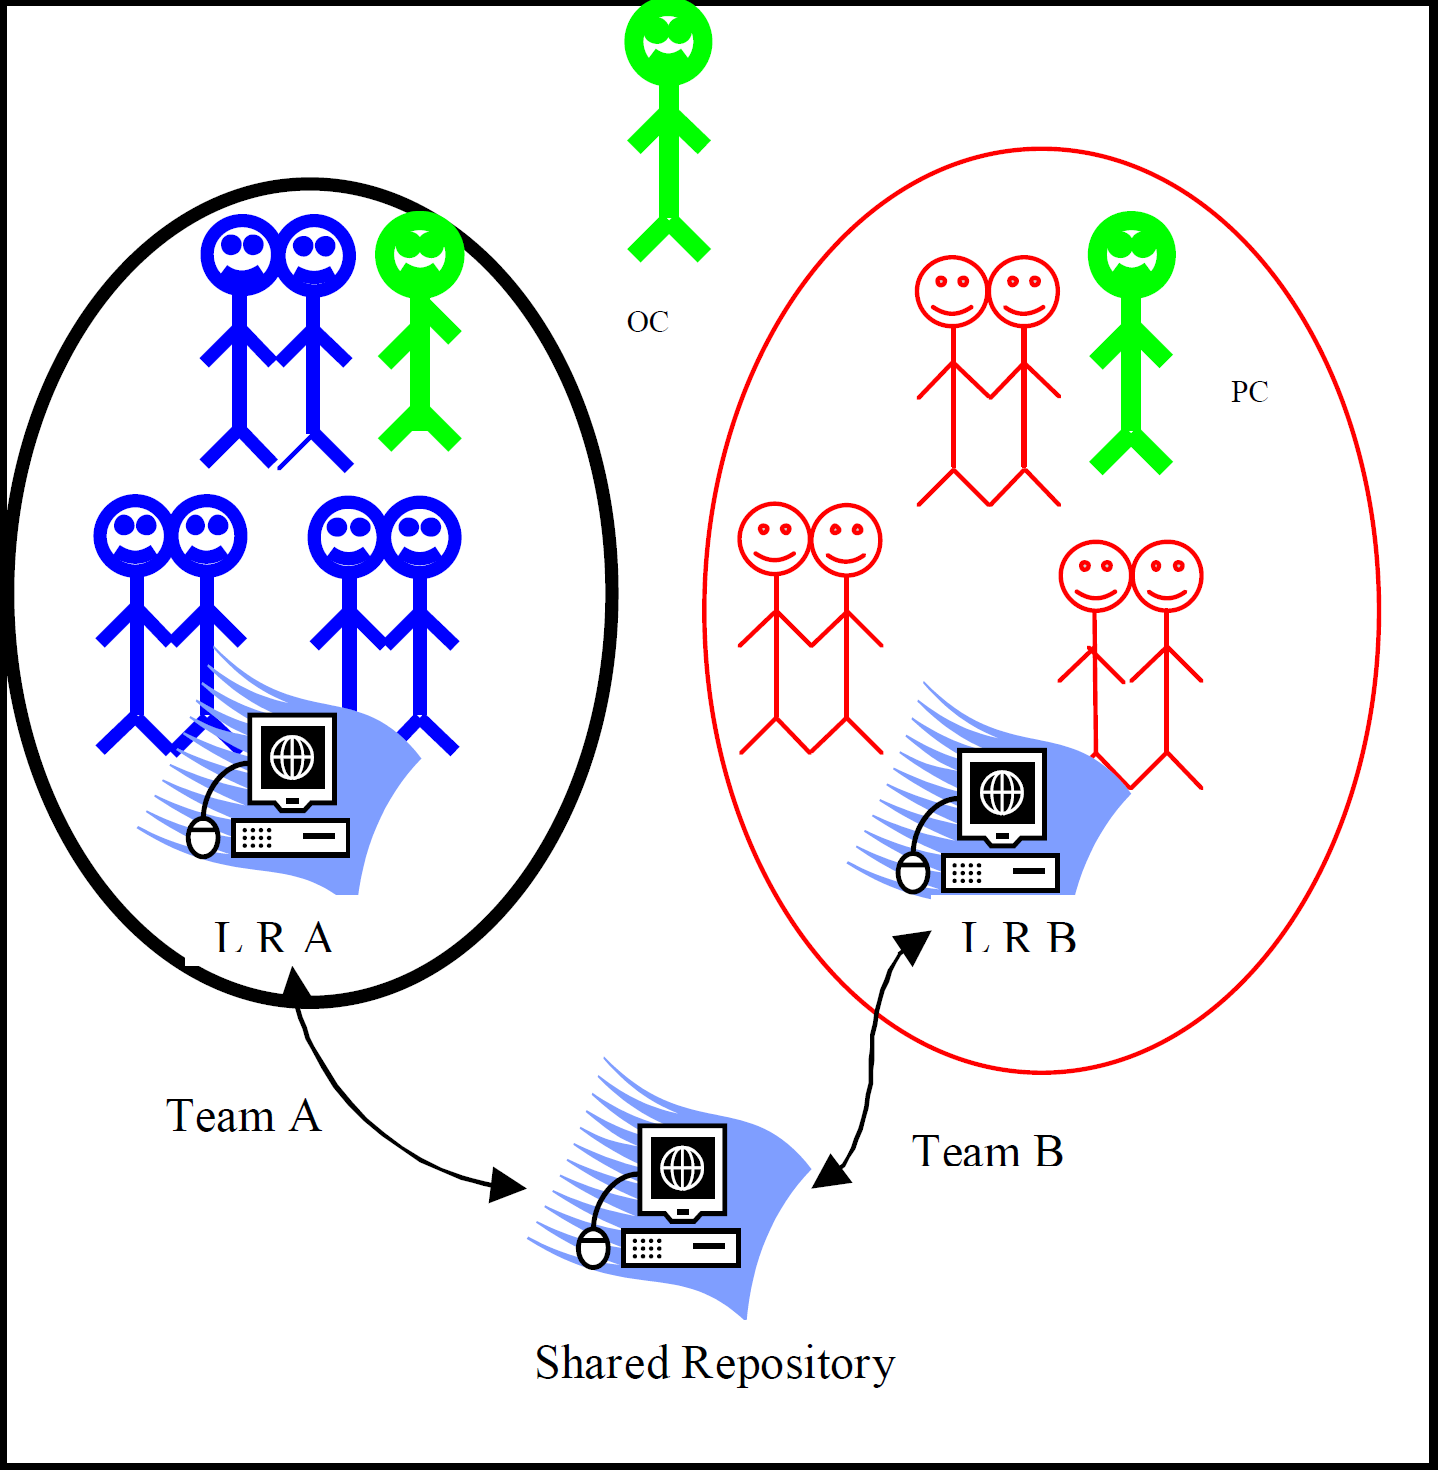
\includegraphics[width=0.8\textwidth]{ACMDSD}
    \caption{Agile Communication Model by Bhalerao\cite{bhalerao2010}}
    \label{fig:ACM}
\end{figure}


Olly Brands talk brings up some interesting points at the Agile-on-the-Beach conference \cite{OllyBrandLiveBlog2015}:

\begin{itemize}
\item Post it notes are key to the agile process and need to be replaced. 
\item Establish a routine and stay organized to be productive. 
\end{itemize}

One great solution to replacing post it notes is online projcet managing software e.g. Trello. This is a ``freemium'' product that allows developers to manage cards containing individual components of the software.

To help developers stay productive, having agreed active and passive forms of communication, such as video conferencing (Active) E-Mail (passive) can improve communication and productivity \cite{joshi2013}. This means that developers can organise a time to do a video conference for every sprint and then use passive forms of communication for the daily scrum.

As Mike Cohn and Doris Ford say, ``bring as many people as possible together for the first week or two of the project can increase the likelihood of success.'' \cite{cohn2003} as the first few weeks of a project normally requires the most amount communication, so having face-to-face communication to get across the overall idea and aim of the project will help reduce confusion later in the project, this is because face-to-face communication is the most effecctive way of conveying information within a development team \cite{williams2012}.

Shared online respitory(GitHub)



\section{Conclusion}

Agile development for distributed teams brings up a lot of communication problems, however to help improve this communication this paper recomends to use Bhaleraos Agile Communication Model \cite{bhalerao2010} with active and 

%References:
%\cite{bhalerao2010}
%\cite{scharff2012}
%\cite{abdullah2011}
%\cite{joshi2013}
%\cite{krasteva2008}
%\cite{williams2012}
%\cite{marjaie2011}
%\cite{kumar2015}
%\cite{cohn2003} https://www.mountaingoatsoftware.com/articles/introducing-an-agile-process-to-an-organization
%\cite{OllyBrandLiveBlog2015}

\bibliographystyle{ieeetr}
\bibliography{comp150_Agile}

\end{document}
